%
% LaTeX report template 
%
\documentclass[a4paper,10pt]{article}
\usepackage{graphicx}
\usepackage{subfigure}
\usepackage{hyperref}
\usepackage[english]{babel}
\usepackage[latin1]{inputenc}

\title{SimpleMessenger with Apache Thrift}
\author{Animesh Baranawal}
\begin{document}

\maketitle

\section{Introduction}
The objective is to create a chat messenger service that supports point to point communication, broadcasts and file sharing among users. The messenger service uses Apache Thrift[1] for supporting communication across different users. Apache Thrift was chosen because of its cross-language support.
 
 
\section{Methods}
The chat messenger is modeled as a central server node acting as a relay between different users, which are modeled as client nodes. Since Apache Thrift does not support any direct 2-way communication[2], each client node runs a mini, light weight server on its side. Java Swing is used as the supporting user-interface framework, and the back-end services are implemented in Java respectively.

\subsection{Basic Structures}
\begin{itemize}
    \item \textbf{UserDefinition}: string uniqueID, string ip\_addr, i32 port
    \item \textbf{GroupDefinition}: string groupID, list\texttt{<}string\texttt{>} members
    \item \textbf{Message}: i64 timestamp, string msgString, string toID, string fromID, bool multicast
    \item \textbf{FileDefinition}: binary data, string fileID, i32 size
    \item \textbf{FileChunk}: binary data, i32 size, i32 offset
\end{itemize}

\subsection{Backend Services}
\begin{itemize}
    \item \textbf{ServerService}: It is hosted by central server for message communication. It supports the following RPC methods: \textit{join}, \textit{connectTo}, \textit{sendMessage}, \textit{joinGroup}, \textit{leaveGroup}. It also spawns dispatcher threads which empty the server message queue.
    \item \textbf{FileTransferService}: It is hosted by central server for file communication. it supports the following RPC methods: \textit{startUpload}, \textit{uploadChunk}, \textit{endUpload}, \textit{startDownload}, \textit{downloadChunk}.
    \item \textbf{ClientService}: It is hosted by client for communication from server. It supports the following RPC methods: \textit{receive}. It also spawns a receiver thread which empties the client message queue.
\end{itemize}

\subsection{Implementation}
\begin{itemize}
    \item Messaging: The client node calls \textit{sendMessage} on ServerService. The server on receiving the message adds it to its message queue. In case the message is to be multicasted to a group, the message is replicated for different user members and then added to the queue. The dispatcher thread takes a message from the server message queue and calls \textit{receive} on the target client node. The ClientService on receiving the message adds it to its message queue. The client receiver thread takes a message from the message queue and passes it to the respective UI widget for displaying.
    \begin{figure}[h]
        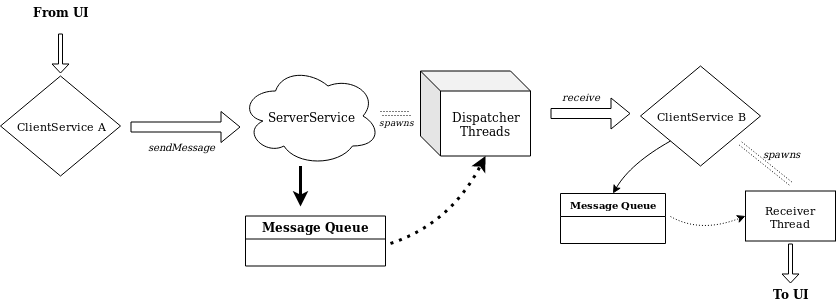
\includegraphics[scale=0.4]{messageWorkflow}
        \caption{Visual description of messaging workflow}
        \label{fig:diagram1}
    \end{figure}
    
    \item FileTransfer: The file transfer workflow is similar to the workflow used in WhatsApp. The client starts uploading by calling \textit{startUpload} on FileTransferService and then uploads the file in chunks of 2048 bytes using \textit{uploadChunk}, followed by an \textit{endUpload} call. This stores the file on the server storage. The client then sends a message to recipient node with the file name. The recipient client calls \textit{startDownload} on FileTransferService followed by \textit{downloadChunk} calls to download the file.
    \begin{figure}[h]
        \hspace{1cm}
        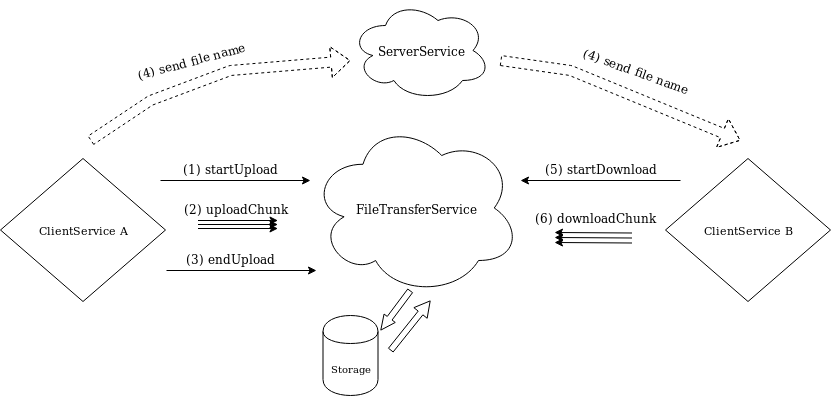
\includegraphics[scale=0.35]{FileTransferWorkflow}
        \caption{Visual description of file transfer workflow}
        \label{fig:diagram2}
    \end{figure}
    
\end{itemize}

\section{Results}
\subsection{Validation}
\texttt{java.util.logging} was used for creating logs of ClientService and ServerService. Every message sent and received by the client is logged along with the sender unique identifier, receiver unique identifier, sent time-stamp and received time-stamp. Latency is measured by calculating the difference between the sent timestamp and received timestamp. Time-stamps for when file upload/download request was sent and when the upload/download got completed are also logged. File transfer time is calculated as the difference of these two timestamps. \par For scenario 1 and 2, simulations were done on a single machine with the server and clients using different port numbers for running the services. The average of maximum latency observed across simulations is used for plotting results. For scenario 3, 2 VMs are set up for simulating clients with original machine simulating the server. 

\subsubsection{Scenario 1: P2P communication}
N different users communicate point to point with each other in this scenario. To validate this scenario, each sent message in the sending client log is checked in the log of the recipient client node.
The simulation was run for N=2,5,10,15,20,25 with the server running 1 dispatcher thread. Figure 3 shows the latency observed. This scenario was simulated 10 times.

\subsubsection{Scenario 2: Multicast communication}
To simulate this scenario, N different users first join a chatroom. Every message sent to the chatroom will be multicasted to all the other user members. To validate this scenario, the list of messages received by a client node was compared to the list of messages sent by all the other client nodes. The scenario was simulated for N=2,5,10,15 with the server running T=1,2,3,5,7 dispatcher threads. Figure 4 shows the latency observed. This scenario was simulated 10 times.

\begin{figure}[!h]
    \hspace{-1.7cm}
    \begin{minipage}[t]{8cm}
	    \centering
		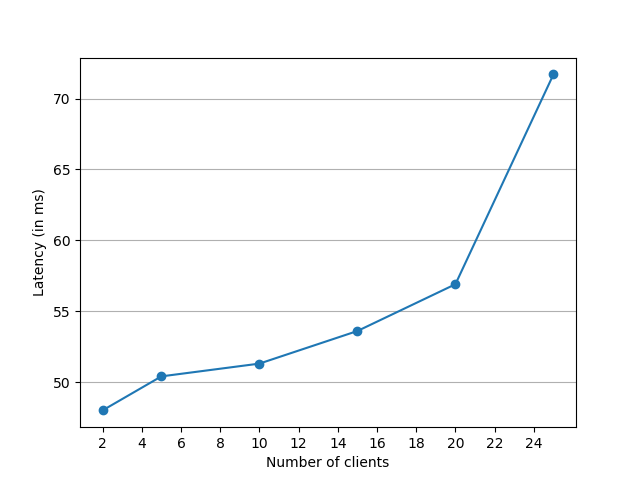
\includegraphics[scale=0.38]{P2P_t1}
		\caption{P2P Latency}
		\label{fig:Diagram3}
	\end{minipage}
	\hspace{-1.5cm}
	\begin{minipage}[t]{10cm}
	    \centering
		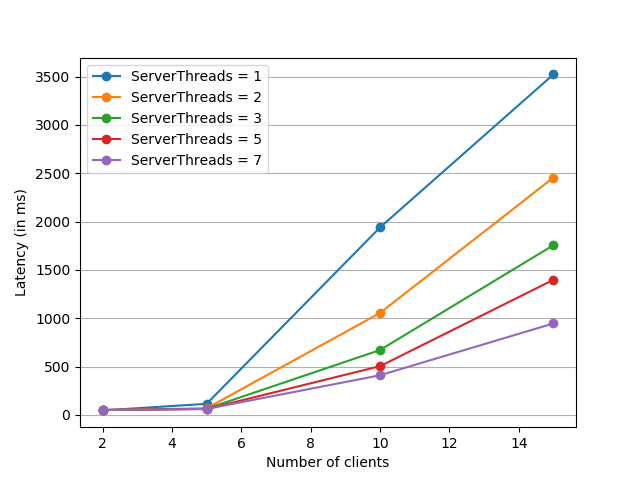
\includegraphics[scale=0.38]{Room_tAll}
		\caption{Multicast Latency}
		\label{fig:Diagram4}
	\end{minipage}
\end{figure}

\subsubsection{Scenario 3: File Transfer between 2 clients}
2 clients simulated by two VMs join the server and transfer file of sizes S = 1,10,100,1000,10000 Kb between them respectively. The scenario was simulated 5 times. To validate, \texttt{diff} was taken between the sent file and received file to find differences if any. Figure 5 shows the average file transfer time across the simulations.
\begin{figure}[h]   
    \hspace{2cm}
    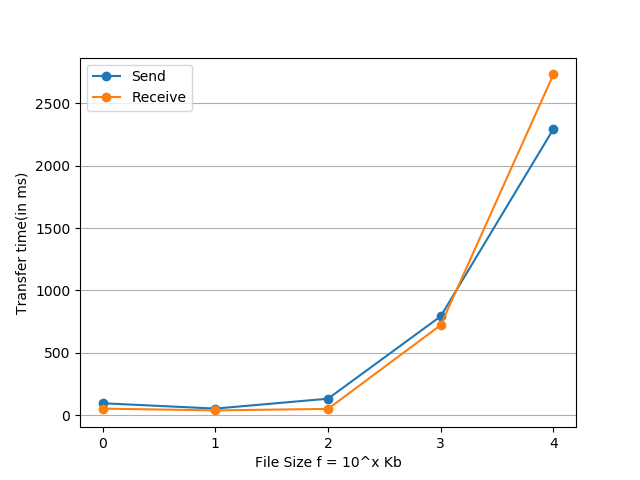
\includegraphics[scale=0.5]{fileTransfer_5Readings}
    \caption{File transfer time for different file sizes}
    \label{fig:diagram2}
\end{figure}

\section{Conclusion}
We developed a simple messenger service using Apache thrift supporting point to point and multicast communication with file sharing. However, the work can be easily extended. \par An extension of the work could be to incorporate fault-tolerance in the application which has not been addressed in either the implementation or scenario simulation. Validation can also be extended to check if the order of messages sent at the sender client node and received at the recipient client node match. Recording the chat conversations to restore the history is yet another extension.

\begin{thebibliography}{}
    \bibitem{thrift} Apache Thrift: \url{https://thrift.apache.org/}
    \bibitem{2-way} \href{http://mail-archives.apache.org/mod\_mbox/thrift-user/201010.mbox/\%3CAANLkTi=Mt4A2YhcDy0GA7pY52O7jSTWmqEoh1E=HzEbw@mail.gmail.com\%3E}{How to send a message from Thrift server to client?}
    \bibitem{URL1} \href{https://sookocheff.com/post/thrift/so-you-want-to-use-thrift/}{So you want to send a message using Apache Thrift?}
    \bibitem{URL2} \href{https://medium.com/codingurukul/whatsapp-engineering-inside-1-1ef4845ff784}{Medium: WhatsApp-Engineering}
    \bibitem{URL3} \href{https://stackoverflow.com/questions/20960541/file-transport-between-server-client}{File Transport between Server/Client using Apache Thrift}
\end{thebibliography}

\end{document}
